\documentclass[10pt]{article}

\usepackage{times}
\usepackage{amsmath}
\usepackage{amssymb}

\usepackage{amsthm}
\theoremstyle{plain}
\newtheorem{definition}{Definition}
\newtheorem{corollary}{Corollary}

\usepackage[en-GB]{datetime2}
\DTMlangsetup[en-GB]{ord=omit}

\usepackage{url}
\urlstyle{rm}

\usepackage[ruled,vlined,linesnumbered]{algorithm2e}
\SetKwFor{ForEach}{for each}{do}{end}
\SetKwProg{Function}{function}{}{}
\SetKwProg{Procedure}{procedure}{}{}
\SetKwProg{Class}{class}{}{}
\SetKwInput{Persistent}{persistent}{}{}
\SetKwInput{Input}{input}{}{}
\SetKwIF{WithProbability}{}{Else}{with probability}{do}{}{else}{end with}
\SetKw{Break}{break}
\DontPrintSemicolon

\usepackage{graphicx}

\usepackage{bm}
\newcommand{\vect}[1]{\bm{#1}}

\usepackage{forest}
\usepackage{tikz}
\usepackage{subcaption}

\DeclareMathOperator*{\argmax}{\arg\!\max}

\usepackage{mdframed}
\usepackage{xcolor}
\newenvironment{note}[1][Note]{
    \begin{center}
    	\begin{minipage}{0.9\linewidth}
    		\begin{mdframed}[backgroundcolor=yellow!25,linewidth=0pt]
    			\textbf{#1:} }{
    		\end{mdframed}
    	\end{minipage}
    \end{center}
}

\title{Simulator-Based Verification of Autonomous Vehicles: Agent-Based Test Generation}
\author{}
\date{\DTMcurrenttime, \today}

\begin{document}

\maketitle

\section{Preliminaries}
We rely on some standard mathematical notation:
$v_{i}$ is an element of vector $\vect{v} = (v_{1}, \dots, v_{n})$ with $\vect{v}_{-i} = (v_{1}, \dots, v_{i-1}, v_{i+1}, \dots, v_ {n})$ the subvector of $\vect{v}$ excluding~$v_{i}$,
$|S|$ is the cardinality of set $S$,
$2^{S}$ is the powerset of $S$,
$\Delta(S)$ is the set of probability distributions over $S$,
$\mathbb{R}$ is the set of real numbers with $\mathbb{R}^{\ge 0}$ is the set of non-negative real numbers,
$\mathbb{Z}^{\ge 0}$ is the set of non-negative integers, and
$\mathbb{N}$ is the set of natural numbers.
A function $f : X \to Y$ is a surjection if for each $y \in Y$ there exists some $x \in X$ such that $f(x) = y$.
Given a function $f : X \to Y$, the inverse image of function $f$ is a function $f_{1}^{-1} : Y \to 2^{E}$ defined as $f_{1}^{-1}(y) = \{ x \in X \mid f(x) = y \}$ for each $y \in Y$.

\subsection{Normal-Form Games}
A normal-form game is a tuple $(N, A, \vect{u})$ where $N = \{ 1, \dots, n \}$ is a finite set of players, $A = A_{1} \times \dots \times A_{n}$ is a set of action profiles with $A_{i}$ the set of actions available to player $i \in N$, and $\vect{u} = (u_{1}, \dots, u_{n})$ is a profile of utility functions with $u_{i} : A \to \mathbb{R}$ the utility function for~$i$.
A (mixed) strategy for player $i \in N$ is a probability distribution $\psi \in \Delta(A_{i})$ with $\vect{\psi} \in \Delta(A_{1}) \times \dots \times \Delta(A_{n})$ a (mixed) strategy profile.
A strategy $\psi$ for player $i \in N$ is a pure strategy if $\psi(a) = 1$ for some $a \in A_{i}$.
A strategy profile $\vect{\psi}$ is a pure strategy profile if $\psi_{i}$ is a pure strategy for each $i \in N$.
For convenience, we may denote a pure strategy $\psi$ for player $i \in N$ directly by the action $a \in A_{i}$ such that $\psi(a) = 1$.
Likewise, we may denote a pure strategy profile $\vect{\psi}$ directly by the action profile $\vect{a} \in A$ such that $\psi_{i}(a_{i}) = 1$ for each player $i \in N$.
The expected utility of a strategy profile $\vect{\psi}$ is then defined as:
\begin{equation*}
	u_{i}(\vect{\psi}) = \sum_{\vect{a} \in A} u_{i}(\vect{a}) \prod_{j \in N} \psi_{j}(a_{j})
\end{equation*}
In game theory, a solution concept is a prediction of how a game will be played.
Solution concepts are typically based on the idea that each player will try to maximise their expected utility under the assumption that other players will do the same.
A feasible deviation from strategy profile $\vect{\psi}$ by player $i \in N$ is a strategy profile $\vect{\psi'} = (\vect{\psi}_{-i}, \psi')$ where $\psi'$ is a strategy for $i$.
A strategy profile $\vect{\psi}$ is a Nash equilibrium if no player $i \in N$ has a feasible deviation $\vect{\psi'}$ from $\vect{\psi}$ such that $u_{i}(\vect{\psi'}) > u_{i}(\vect{\psi})$.
Every normal-form game with a finite set of players and a finite set of action profiles is guaranteed to have at least one (not necessarily pure) Nash equilibrium~\cite{Nash:AM:1951}.

\subsection{Markov Games}
A (fully observable) Markov game is a tuple $(N,$ $S, A, T, \vect{R})$ where
$N = \{ 1, \dots, n \}$ is a finite set of players,
$S$ is a set of states,
$A = A_{1} \times \dots \times A_{n}$ is a set of action profiles with $A_{i}$ the set of actions available to player $i \in N$,
$T : S \times A \to \Delta(S)$ is a (stochastic) transition function, and
$\vect{R} = (R_{1}, \dots, R_{n})$ is a profile of reward functions with $R_{i} : S \to \mathbb{R}$ the reward function for player $i \in N$.
A Markov game is zero-sum if $\sum_{i \in N} R_{i}(s) = 0$ for each state $s \in S$.

A Markov game is composed of a sequence of normal-form games, called stage games, where players seek to optimise their return for the whole game rather than for individual stage games.
The current stage game is determined by the current state, and players transition between states by executing action profiles.
The game is said to be fully observable because players are assumed to observe the current (shared) state at each decision step.
Let $T(s, \vect{a}, s')$ denote the probability of transitioning to state $s' \in S$ after executing action profile $\vect{a} \in A$ in state $s \in S$ according to probability distribution $T(s, \vect{a})$.
The probability of transitioning to state $s' \in S$ after executing strategy profile $\vect{\psi}$ in state $s \in S$ is:
\begin{equation*}
    T(s, \vect{\psi}, s') = \prod_{\vect{a} \in A} T(s, \vect{a}, s') \prod_{j \in N} \psi_{j}(a_{j})
\end{equation*}
The stage game for state $s \in S$ is a normal-form game $(N, A, \vect{u})$ where the utility function $u_{i}$ for player $i \in N$ is defined for each action profile $\vect{a} \in A$ as the immediate expected reward:
\begin{equation*}
    u_{i}(\vect{a}) = \sum_{s' \in S} T(s, \vect{a}, s') R_{i}(s')
\end{equation*}
Markov games subsume several other important frameworks: a Markov game is a repeated game if $|S| = 1$, and is a Markov decision process (MDP) if $|N| = 1$.

Solutions to Markov games are represented as functions, called policies, that map \emph{histories} to strategies.
An execution is a possibly infinite sequence $(s_{1}, \vect{a}_{1}, s_{2}, \vect{a}_{2}, \dots)$ of states and action profiles.
A history of length $t$ is a finite execution $h_{t} = (s_{1}, a_{1},$ $\dots, a_{t-1}, s_{t})$ ending in a state.
Let $H_{t}$ be the set of histories of length $t$ with $D = \{ 1, 2, \dots, t_{\max} \}$ the set of decision-steps up to horizon $t_{\max} \in \mathbb{N} \cup \{ \infty \}$ and $H = \{ h \in H_{t} \mid t \in D \}$ the set of histories up to $t_{\max}$.
A (stochastic or mixed) policy for player $i \in N$ is a function $\pi_{i} : H' \to \Delta(A_{i})$ where $H' \subseteq H$.
Let $\pi_{i}(h, a)$ denote the probability that player $i \in N$ should execute action $a \in A_{i}$ in history $h \in H'$ according to strategy $\pi_{i}(h)$.
A policy $\pi_{i}$ for player $i \in N$ is a deterministic (or pure) policy if $\pi_{i}(h, a) = 1$ for each $h \in H'$ and some $a \in A_{i}$.
A policy $\pi_{i}$ for player $i \in N$ is state-based if $\pi_{i}(h_{t}) = \pi_{i}(h_{t'})$ for all $h_{t}, h_{t'} \in H'$ such that $t = t'$ and $s_{t} = s_{t'}$.
A state-based policy for player $i \in N$ may be written as $\pi_{i} : X \to \Delta(A_{i})$ where $X \subseteq S \times D$.
A state-based policy $\pi_{i}$ for player $i \in N$ is stationary if $\pi_{i}(s, t) = \pi_{i}(s, t')$ for all $(s, t), (s, t') \in X$, otherwise $\pi_{i}$ is non-stationary.
A stationary state-based policy for player $i \in N$ may be written as $\pi_{i} : S' \to \Delta(A_{i})$ where $S' \subseteq S$.
A tuple $\vect{\pi} = \left( \pi_{1}, \dots, \pi_{n} \right)$ is a policy profile (resp.\ deterministic policy profile) if each $\pi_{i}$ is a policy (resp.\ deterministic policy) over $H' \subseteq H$.
The strategy profile for history $h \in H'$ according to policy profile $\vect{\pi}$ is $\vect{\pi}(h) = \left( \pi_{1}(h), \dots, \pi_{n}(h) \right)$.

Solutions are only well-defined for certain classes of Markov game.
Two standard examples are finite-horizon Markov games and infinite-horizon (discounted reward) Markov games.
A finite-horizon Markov game is a tuple $(\Gamma, t_{\max})$ where $\Gamma$ is a Markov game and $t_{\max} \in \mathbb{N}$ is a horizon.
An infinite-horizon Markov game is a tuple $(\Gamma, \gamma)$ where $\Gamma$ is a Markov game and $0 \le \gamma < 1$ is a discount factor.
It is known that attention can be restricted to stationary state-based policies in the case of infinite-horizon Markov games, and to non-stationary state-based policies in the case of finite-horizon Markov games.
Depending on context, we will assume hereafter that all policies are either stationary or non-stationary state-based policies.
For an infinite-horizon Markov game $(\Gamma, \gamma)$, the expected value of policy profile $\vect{\pi}$ for player $i \in N$ in state $s \in S$ is:
\begin{equation*}
    V_{i}(\vect{\pi}, s) = \sum_{s' \in S} T(s, \vect{\pi}(s), s') \left[ R_{i}(s') + \gamma V_{i}(\vect{\pi}, s') \right]
\end{equation*}
For a finite-horizon Markov game $(\Gamma, t_{\max})$, the expected value of policy profile $\vect{\pi}$ for player $i \in N$ in state $s \in S$, with $t \in D \cup \{ 0 \}$ remaining decision-steps, is:
\begin{align*}
    V_{i}(\vect{\pi}, s, t) =
    \begin{cases}
        \sum\limits_{s' \in S} T(s, \vect{\pi}(s, t), s') \left[ R_{i}(s') + V_{i}(\vect{\pi}, s', t-1) \right] & \text{if $t > 0$} \\
        0 & \text{if $t = 0$}
    \end{cases}
\end{align*}
A feasible deviation from policy profile $\vect{\pi}$ by player $i \in N$ is a policy profile $\vect{\pi'} = (\vect{\pi}_{-i}, \pi')$ where $\pi'$ is a policy for $i$.
A policy profile $\vect{\pi}$ is a Nash equilibrium if no player $i \in N$ has a feasible deviation $\vect{\pi'}$ from $\vect{\pi}$ such that $V_{i}(h, \vect{\pi'}) > V_{i}(h, \vect{\pi})$ for each $h \in H'$.

\newpage
\section{Framework}\label{section:framework}

\begin{definition}\label{definition:architecture}
    A (simulator-based) test generation architecture is a tuple $(N, M, E,$ $f_{1}, f_{2})$ where:
    \begin{itemize}
        \item $N = \{ 1, \dots, n \}$ is a set of agents such that $n \ge 2$ with $1 \in N$ the ego agent (or design under test)
        \item $M$ is a set of actors with $f_{1} : M \to N$ a surjection mapping actors to agents
        \item $E$ is a set of effectors with $f_{2} : E \to M$ a surjection mapping effectors to actors and $A(e)$ the non-empty set of actions available to effector $e \in E$
    \end{itemize}
\end{definition}

\begin{corollary}
    $2 \le |N| \le |M| \le |E|$.
\end{corollary}

\begin{figure}[t]
    \centering
    \scriptsize
    \begin{forest}
        for tree={s sep=-1pt},
        if level=0{l sep+=10pt}{},
        [MAS
            [Agent, label={above left:\emph{Design under Test}}
                [Actor [Effector] [$\dots$] [Effector]]
                [$\dots$ [$\dots$]]
                [Actor [Effector] [$\dots$] [Effector]]
            ]
            [$\dots$
                [$\dots$ [$\dots$]]
            ]
            [Agent, label={above right:\emph{Test Generator}}
                [Actor [Effector] [$\dots$] [Effector]]
                [$\dots$ [$\dots$]]
                [Actor [Effector] [$\dots$] [Effector, edge label={node[midway,above right]{\emph{Simulator}}}]]
            ]
        ]
        \draw (-5.25, -0.25) [dotted] rectangle (-2, -1.2);
        \draw (-0.5, -0.25) [dotted] rectangle (4.9, -1.2);
        \draw (-5.75, -1.3) [dotted] rectangle (6, -2.5);
    \end{forest}
    \caption{Architecture for agent-based test generation}
    \label{figure:architecture}
\end{figure}

The set of actors associated with agents $N' \subseteq N$ is defined as $M(N') = \{ m \in f_{1}^{-1}(i) \mid i \in N' \}$.
The set of effectors associated with actors $M' \subseteq M$ is defined as $E(M') = \{ e \in f_{2}^{-1}(m) \mid m \in M' \}$.
The set of joint actions available to effectors $E' \subseteq E$ is defined as $A(E') = \times_{e \in E'} A(e)$.
Definition~\ref{definition:architecture} is visualised in Figure~\ref{figure:architecture}, with the set of actors $M$ (resp.\ agents $N$) inducing a partition of the set of effectors $E$.

\begin{definition}\label{definition:game}
    A (simulator-based) test generation game is a tuple $(G, S, A, T, \vect{R})$:
    \begin{itemize}
        \item $G = (N, M, E, f_{1}, f_{2})$ is a test generation architecture
        \item $(N, S, A, T, \vect{R})$ is a Markov game such that $A_{i} = A(E(M(\{ i \})))$ is the set of actions available to agent $i \in N$
    \end{itemize}
\end{definition}

\begin{definition}
    A test generation game $(G, S, A, T, \vect{R})$ is collaborative if $R_{i}(s) = R_{j}(s)$ for all $i, j \in N \setminus \{ 1 \}$ and each $s \in S$.
\end{definition}

Simulator-based test generation constitutes a multi-agent system because it involves a group of (one or more) tester agents playing against a single ego agent: the former is under the control of the test generation system, while the latter is not.
The objective of simulator-based test generation is then to design a group of tester agents so as to influence the ego agent towards achieving some test goal.
Definition~\ref{definition:game} formally models this problem as a Markov game (also known as a stochastic game).
Markov games assume that time is composed of discrete decision steps in which agents execute actions simultaneously.
Although the transition function $T$ and reward functions $\vect{R}$ are specified in Definition~\ref{definition:game}, these may be unknown in practice (as is the case in multi-agent reinforcement learning).
What is important is that a simulator provides feedback to agents in a way that constitutes sampling from $T$ and $\vect{R}$, allowing agents to approximate $T$ and $\vect{R}$ through interaction with the simulator.

\begin{definition}
    Let $\pi_{1}$ be a deterministic policy and $\omega \subseteq S$ be a (test) assertion.
    An interesting test given $\pi_{1}$ and $\omega$ is a tuple $(s_{1}, \vect{\pi}_{-1})$ where $s_{1} \in S$ is an initial state and $\vect{\pi}_{-1}$ is a deterministic policy profile for the set of agents $N \setminus \{ 1 \}$ such that executing policy profile $(\pi_{1}, \vect{\pi}_{-1})$ in state $s_{1}$ leads to some state $s \in \omega$ within a finite number of timesteps.
\end{definition}

\begin{note}
    Assertions could be generalised to sequences of states (e.g.\ using a termporal logic?) or to executions (e.g.\ with actions as events?).
\end{note}

\begin{note}
    We assume that a stochastic policy is always fixed to a deterministic policy by controlling the seed, but this means the test is only interesting with respect to that seed.
    Is there a more general notion?
\end{note}

\begin{note}
    How to \emph{repeat} a test when a different ego policy $\pi_{1}'$ may cause the assertion to be avoided altogether (e.g.\ by causing the agents to arrive in history $h \in H$ such that $\vect{\pi}_{-1}$ is undefined for $h$)?
\end{note}

\newpage
\section{Experiments}\label{section:case-study}

\begin{figure}[tbph]
    \scriptsize
    \begin{subfigure}{\linewidth}
        \centering
        \begin{forest}
            for tree={s sep=-1pt},
            if level=0{l sep+=10pt}{},
            [MAS
                [AV, label={above left:\emph{Design under Test}}
                    [Vehicle [Acceleration] [Steering]]
                ]
                [Agent
                    [Pedestrian [Acceleration] [Steering]]
                ]
                [$\dots$
                    [$\dots$ [$\dots$]]
                ]
                [Agent, label={above right:\emph{Test Generator}}
                    [Pedestrian [Acceleration] [Steering, edge label={node[midway,above right]{~~~~~\emph{Simulator}}}]]
                ]
            ]
            \draw (-4.9, -0.25) [dotted] rectangle (-2, -1.2);
            \draw (-0.75, -0.25) [dotted] rectangle (4.6, -1.2);
            \draw (-4, -1.3) [dotted] rectangle (4.4, -2.5);
        \end{forest}
        \caption{$n$ single-actor agents}
    \end{subfigure}
    \begin{subfigure}{\linewidth}
        \centering
        \begin{forest}
            for tree={s sep=-1pt},
            if level=0{l sep+=10pt}{},
            [MAS
                [AV, label={above left:\emph{Design under Test}}
                    [Vehicle [Acceleration] [Steering]]
                ]
                [Agent, label={above right:\emph{Test Generator}}
                    [Pedestrian [Acceleration] [Steering]]
                    [$\dots$ [$\dots$]]
                    [Pedestrian [Acceleration] [Steering, edge label={node[midway,above right]{~~~~~\emph{Simulator}}}]]
                ]
            ]
            \draw (-4.15, -0.25) [dotted] rectangle (-1.25, -1.2);
            \draw (1, -0.25) [dotted] rectangle (3.85, -1.2);
            \draw (-3.3, -1.3) [dotted] rectangle (5.15, -2.5);
        \end{forest}
        \caption{$1$ multi-actor agent}
    \end{subfigure}
    \caption{Agent-based test generation in \textsc{CAV-Gym:Pedestrians}}
\end{figure}

\begin{figure}[htbp]
    \centering
    \frame{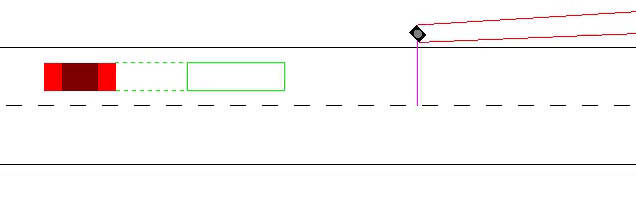
\includegraphics[width=\textwidth]{figures/cav-gym-cropped}}
    \caption{\textsc{CAV-Gym:Pedestrians}}
    \label{figure:cav-gym}
\end{figure}

\begin{algorithm}[htbp]
	\caption{\textsc{Simulator}}
	\label{algorithm:simulation}
	\footnotesize
    \Persistent{environment $e$, agents $N = \{ 1, \dots, n \}$, terminator $\psi \subseteq S$}
    \Begin{
        \ForEach{episode}{
            $s \leftarrow$ reset $e$\;
            \ForEach{timestep}{
                $\vect{a} \leftarrow \left( \textsc{ChooseAction}_{1}(s), \dots, \textsc{ChooseAction}_{n}(s) \right)$\;
                $\vect{r}, s' \leftarrow$ execute $\vect{a}$ in $e$\;
                \ForEach{agent $i \in N$}{$\textsc{ProcessFeedback}_{i}(s, a_{i}, r_{i}, s')$}
                \leIf{$s' \in \psi$}{\Break}{$s \leftarrow s'$}
            }
        }
    }
\end{algorithm}

\begin{algorithm}[p]
	\caption{\textsc{RandomAgent}}
	\label{algorithm:random_agent}
	\footnotesize
    \Persistent{exploration rate $\epsilon \in [0, 1]$}
    \Function{$\textsc{ChooseAction}(s)$}{
        \WithProbability{$\epsilon$}{
            \Return random choice from $A(s)$
        }
        \Return $\varnothing$
    }
\end{algorithm}

\begin{algorithm}[p]
	\caption{\textsc{ProgrammedRandomAgent}}
	\label{algorithm:random_constrained_agent}
	\footnotesize
    \Persistent{programmed behaviour $\pi : S \to A$, terminator $\psi \subseteq S$, exploration rate $\epsilon \in [0, 1]$}
    \Function{$\textsc{ChooseAction}(s)$}{
        \If{$\pi$ is active}{
            \leIf{$s \in \psi$}{set $\pi$ as inactive}{\Return $\pi(s)$}
        }
        \WithProbability{$\epsilon$}{
            set $\pi$ as active\;
            \Return $\pi(s)$
        }
        \Return $\varnothing$
    }
\end{algorithm}

\begin{algorithm}[p]
	\caption{\textsc{ProgrammedReactiveAgent}}
	\label{algorithm:proximity_agent}
	\footnotesize
    \Persistent{programmed behaviour $\pi : S \to A$, trigger $\varphi \subseteq S$, terminator $\psi \subseteq S$}
    \Function{$\textsc{ChooseAction}(s)$}{
        \If{$\pi$ is active}{
            \leIf{$s \in \psi$}{set $\pi$ as inactive}{\Return $\pi(s)$}
        }
        \If{$s \in \varphi$}{
            set $\pi$ as active\;
            \Return $\pi(s)$
        }
        \Return $\varnothing$
    }
\end{algorithm}

\begin{algorithm}[p]
	\caption{\textsc{ProgrammedElectionAgent}}
	\label{algorithm:election_agent}
	\footnotesize
    \Persistent{programmed behaviour $\pi : S \to A$, terminator $\psi \subseteq S$, coordinator $c$}
    \Function{$\textsc{ChooseAction}(s)$}{
        \If{$\pi$ is active}{
            \leIf{$s \in \psi$}{set $\pi$ as inactive}{\Return $\pi(s)$}
        }
        \If{elected by $c$}{
            set $\pi$ as active\;
            \Return $\pi(s)$
        }
        \Return $\varnothing$
    }
\end{algorithm}

\begin{algorithm}[p]
	\caption{\textsc{QLearningAgent}}
	\label{algorithm:qlearning_agent}
	\footnotesize
    \Persistent{learning rate $\alpha \in [0, 1]$, discount factor $\gamma \in [0, 1]$, exploration rate $\epsilon \in [0, 1]$,\newline
    feature $f_{j} : S \times A \to \mathbb{R}$ with weight $w_{j} \in \mathbb{R}$ for $j = 1, \dots, m$}
    \Function{$\textsc{ChooseAction}(s)$}{
        \WithProbability{$\epsilon$}{
            \Return random choice from $A(s)$
        }
        \Return random choice from $\argmax_{a \in A(s)} \textsc{QValue}(s, a)$
    }
    \Procedure{$\textsc{ProcessFeedback}(s, a, r, s')$}{
        $q \leftarrow \left( r + \gamma \cdot \max_{a' \in A(s')} \textsc{QValue}(s', a') \right) - \textsc{QValue}(s, a)$\;
        \ForEach{feature $f_{j}$}{$w_{j} \leftarrow w_{j} + \alpha \cdot q \cdot f_{j}(s, a)$}
    }
    \Function{$\textsc{QValue}(s, a)$}{
        \Return $\sum_{j = 1}^{m} f_{j}(s, a) \cdot w_{j}$
    }
\end{algorithm}

\bibliographystyle{plain}
\bibliography{agent-test-generation}

\end{document}
